\documentclass[12pt,oneside]{exam}

% This package simply sets the margins to be 1 inch.
\usepackage[margin=1in]{geometry}

% These packages include nice commands from AMS-LaTeX
\usepackage{amssymb,amsmath,amsthm,amsfonts,latexsym,verbatim,xspace,setspace}
\usepackage{hyperref}
\usepackage{graphicx}

% Make the space between lines slightly more
% generous than normal single spacing, but compensate
% so that the spacing between rows of matrices still
% looks normal.  Note that 1.1=1/.9090909...
\renewcommand{\baselinestretch}{1.1}
\renewcommand{\arraystretch}{.91}

% Define environments for exercises.
\newenvironment{exercise}[1]{\vspace{.1in}\noindent\textbf{Problem #1 \hspace{.05em}}}{}
\newenvironment{newsolution}{\vspace{.1in}\noindent\textbf{Solution: \hspace{.05em}}}{}

% define shortcut commands for commonly used symbols
\newcommand{\R}{\mathbb{R}}
\newcommand{\C}{\mathbb{C}}
\newcommand{\Z}{\mathbb{Z}}
\newcommand{\Q}{\mathbb{Q}}
\newcommand{\N}{\mathbb{N}}
\newcommand{\calP}{\mathcal{P}}
\DeclareMathOperator{\sech}{sech}
\DeclareMathOperator{\csch}{csch}
\DeclareMathOperator{\vsspan}{span}

\title{Math 514 - Summer II 2020: Quiz 2}

%%%%%%%%%%%%%%%%%%%%%%%%%%%%%%%%%%%%%%%%%%

\begin{document}

\begin{flushright}
\sc MAT 514 - Summer II 2020\\
July 14, 2020
\end{flushright}
\bigskip
 
\begin{center}
\textsf{Quiz 2} 
\end{center}

%%%%%%%%%%%%%%%%%%%%%%%%%%%%%%%%%%%%%%%%

\begin{exercise}{1}
Find the norm and polar angle of the complex number
\begin{equation*}
z=(-3 + \sqrt{3}i)^3
\end{equation*}
\end{exercise}

\textbf{Solution:} The easier way to solve this problem is to find the norm and polar angle of $(-3+\sqrt{3}i)$, and operate with these according to the rules of complex multiplication in polar form. The norm is
\begin{equation*}
|(-3+\sqrt{3}i)| = \sqrt{(-3)^2+(\sqrt{3})^2} = \sqrt{12} = 2\sqrt{3},
\end{equation*}
while the polar angle $\theta$ satisfies
\begin{align*}
\cos(\theta) & = \frac{-3}{2\sqrt{3}}\\
\sin(\theta) & = \frac{\sqrt{3}}{2\sqrt{3}},
\end{align*}
thus $\theta = \frac{5\pi}{6}$. 

In polar form, complex multiplication works by multiplying the norms and adding the polar angles, therefore $z$ has norm
\begin{equation*}
|z| = (2\sqrt{3})^3 = 24\sqrt{3}, 
\end{equation*}
and polar angle 
\begin{equation*}
\phi = 3\theta = \frac{5\pi}{2}. 
\end{equation*}
It is conventional to limit polar angles to $[0,2\pi)$, so we can replace $\frac{5\pi}{2}$ by $\frac{\pi}{2}$, its coterminal angle in the desired range. 


\vfill
\begin{exercise}{2}
Sketch the following set on the complex plane. Determine the following topological properties: is it open? is it closed? is it bounded? is it compact? it is connected?
\begin{equation*}
\{z \in \mathbb{C} | |z+1|+|z-1| < 3\}
\end{equation*}
\end{exercise}
\vfill

\textbf{Solution:} Below is a plot of the region in the complex plane.
\begin{center}
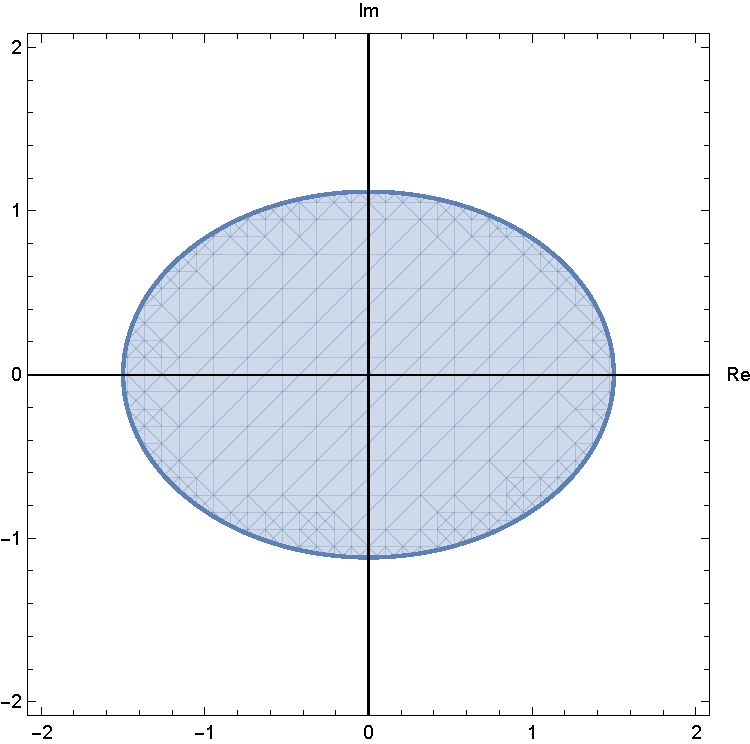
\includegraphics[scale=0.5]{p1.pdf}  
\end{center}

Below we discuss its topological properties:
\begin{itemize}
\item This is an open subset. Indeed, given a point $z$ within it, the disk centered at $z$ whose radius is half the distance between $z$ and the boundary elipse is  entirely contained within this set.
\item It is not closed, as it does not include its boundary points (the elipse).
\item It is bounded, as it is contained in a disk of radius 2 centered at the origin.
\item It is not compact, since it is not closed.
\item It is connected, and in fact convex (any pair of points may be joined by a line segment entirely contained within the set).
\end{itemize}
      
\end{document}

